\sec{Lineární navazovací podmínky}\index{vlnová funkce!sešívání}
V bodech obratu $p(x_{1,2})=0$,\index{bod!obratu} které ohraničují kinematicky dostupnou oblast, vlnová funkce WKB aproximace diverguje.
Vlnová funkce je přitom nenulová vně i uvnitř kinematicky dostupné oblasti, a je proto nutné ji přes bod obratu správně navázat.
To lze provést buď přes komplexní rozšíření souřadnice~\cite{Cejnar2013}, nebo přes aproximaci potenciálu v okolí bodu obratu. 
Pokud $p'(x_{1,2})\neq0$ a zároveň $p'(x)$ je spojitá v bodech $x_{1,2}$, pak se potenciál v okolí bodů obratu aproximuje lineární funkcí, pro kterou je známo přesné řešení Schrödingerovy rovnice ve tvaru Airyho funkcí~\cite{Formanek2004}.\index{funkce!Airyho}

\begin{figure}[!htbp]
    \begin{subfigure}{0.45\linewidth}
        \centering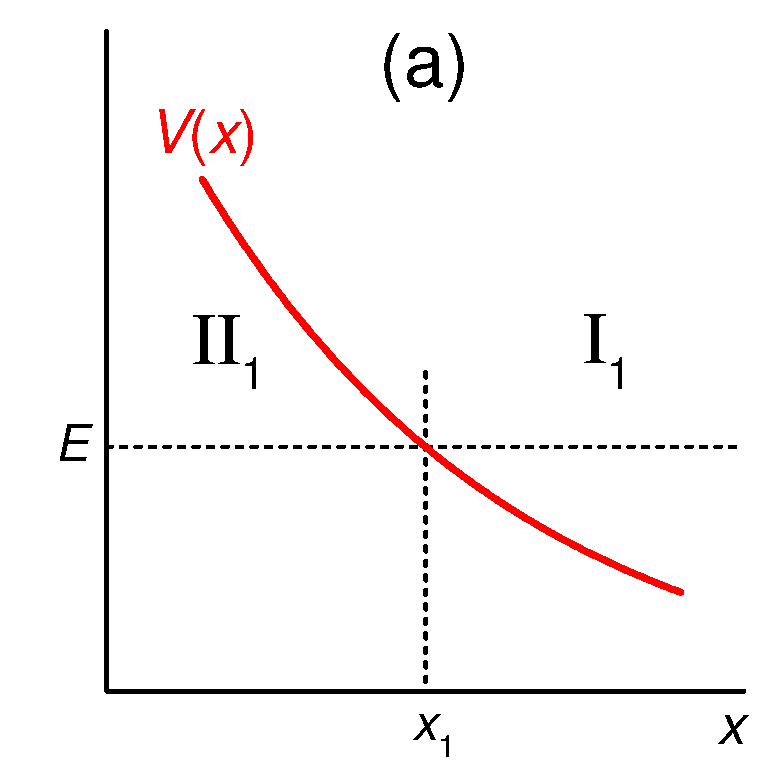
\epsfig{file=wkb_down.eps,width=\linewidth}
    \end{subfigure}
    \hfill
    \begin{subfigure}{0.45\linewidth}
        \centering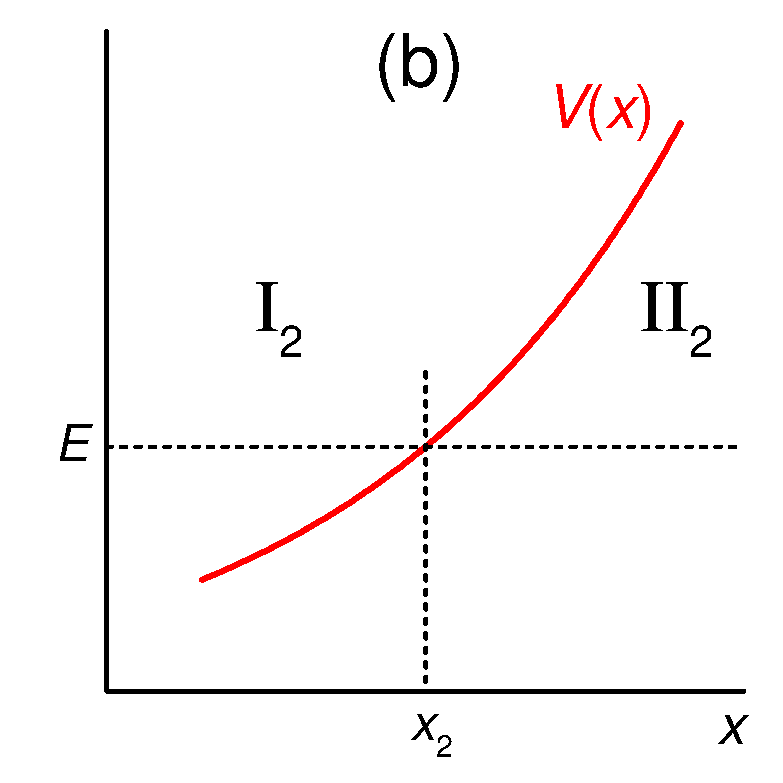
\epsfig{file=wkb_up.eps,width=\linewidth}	
    \end{subfigure}
    \scaption{
        Body obratu pro navazování WKB vlnových funkcí.
    }
\label{fig:WKBConnection}
\end{figure}				

\begin{itemize}
\item
    V bodě obratu $x_{1}$, ve kterém potenciál klesá, $V'(x_{1})<0$, viz obrázek~\ref{fig:WKBConnection}(a), se mění fáze vlnové funkce o $\frac{\pi}{4}$ a zdvojnásobuje se amplituda u sinové části:
    \begin{subequations}
        \begin{align}
            \psi_{\mathrm{II}_{1}}(x)&=\frac{C_{1}}{\sqrt{\abs{p(x)}}}\e^{-\frac{1}{\hbar}\int_{x}^{x_{1}}\abs{p(x')}\d x'},\\
            \psi_{\mathrm{I}_{1}}(x)&=\frac{2C_{1}}{\sqrt{\abs{p(x)}}}\sin\left[\frac{1}{\hbar}\int_{x_{1}}^{x}p(x')\d x'+\frac{\pi}{4}\right]
        \end{align}            
        \label{eq:WKBConnectionDown1}
    \end{subequations}
    a
    \begin{subequations}
        \begin{align}
            \psi_{\mathrm{II}_{1}}(x)&=\frac{C_{1}}{\sqrt{\abs{p(x)}}}\e^{\frac{1}{\hbar}\int_{x}^{x_{1}}\abs{p(x')}\d x'},\\
            \psi_{\mathrm{I}_{1}}(x)&=\frac{C_{1}}{\sqrt{\abs{p(x)}}}\cos\left[\frac{1}{\hbar}\int_{x_{1}}^{x}p(x')\d x'+\frac{\pi}{4}\right],
        \end{align}		            
        \label{eq:WKBConnectionDown2}
    \end{subequations}
    kde oblast II$_{1}$ odpovídá $x<x_{1}$ a oblast I$_{1}$ odpovídá $x>x_{1}$.
    Integrační meze v integrálech jsou zvoleny tak, aby spodní mez byla vždy menší než horní mez, a tedy integrace probíhala postupně zleva doprava.
    
\item
    V bodě obratu $x_{2}$, ve kterém potenciál roste, $V'(x_{2})>0$, viz obrázek~\ref{fig:WKBConnection}(b), je analogicky\footnote{
        Navazovací podmínky~\eqref{eq:WKBConnectionUp1}--\eqref{eq:WKBConnectionUp2} jsou samozřejmě zcela ekvivalentní podmínkám~\eqref{eq:WKBConnectionDown1}--\eqref{eq:WKBConnectionDown2} a zde jsou vypsány jen pro úplnost a pro rychlejší referenci v příkladech.
    }
    \begin{subequations}
        \begin{align}
            \psi_{\mathrm{I}_{2}}(x)&=\frac{2C_{2}}{\sqrt{\abs{p(x)}}}\sin\left[\frac{1}{\hbar}\int_{x}^{x_{2}}p(x')\d x'+\frac{\pi}{4}\right],\\
            \psi_{\mathrm{II}_{2}}(x)&=\frac{C_{2}}{\sqrt{\abs{p(x)}}}\e^{-\frac{1}{\hbar}\int_{x_{2}}^{x}\abs{p(x')}\d x'}\,,
        \end{align}            
        \label{eq:WKBConnectionUp1}
    \end{subequations}
    nebo
    \begin{subequations}
        \begin{align}
            \psi_{\mathrm{I}_{2}}(x)&=\frac{C_{2}}{\sqrt{\abs{p(x)}}}\cos\left[\frac{1}{\hbar}\int_{x}^{x_{2}}p(x')\d x'+\frac{\pi}{4}\right],\\
            \psi_{\mathrm{II}_{2}}(x)&=\frac{C_{2}}{\sqrt{\abs{p(x)}}}\e^{\frac{1}{\hbar}\int_{x_{2}}^{x}\abs{p(x')}\d x'},
        \end{align}            
        \label{eq:WKBConnectionUp2}
    \end{subequations}
    kde oblast I$_{2}$ odpovídá $x<x_{2}$ a oblast II$_{2}$ odpovídá $x>x_{2}$.
\end{itemize}

\sec{Kvadratické navazovací podmínky}
	V případě kvadratické bariéry lze navazující podmínky před a po bariéře vyjádřit například v tomto tvaru:
    \begin{subequations}
        \begin{align}
            \psi_{\mathrm{I}}(x)
                &=C\frac{\e^{-\pi\epsilon}}{\sqrt{p(x)}}
                \e^{\pm\frac{\im}{\hbar}\int_{x}^{a}p(x')\d x'\mp\im\frac{\pi}{4}}
                +C\frac{\sqrt{1+\e^{-2\pi\epsilon}}}{\sqrt{p(x)}}
                \e^{\mp\frac{\im}{\hbar}\int_{x}^{a}p(x')\d x'\pm\im\frac{\pi}{4}}\e^{\pm\im\phi(\epsilon)},
            \psi_{\mathrm{II}}(x)
                &=\frac{C}{\sqrt{p(x)}}
                \e^{\pm\frac{\im}{\hbar}\int_{b}^{x}p(x')\d x'\pm\im\frac{\pi}{4}},
        \end{align}            
    \end{subequations}
	přičemž v případě horních znamének odpovídá první vlna odražené vlně, druhá vlna dopadající vlně a třetí vlna prošlé vlně.
	Dodatečný fázový posun má vyjádření
	\begin{equation}
		\phi(\epsilon)=\epsilon+\arg\Gamma\left(\frac{1}{2}+\im\epsilon\right)-\epsilon\ln\abs{\epsilon}.
	\end{equation}
	Uvedený vztah platí pod i nad bariérou, kdy se do integrálů akce dosadí $c$ namísto $a$ a $b$.
    